\chapter{Tribler, TrustChain and Implementation}
\label{chap:implementation}

Distributed trust systems rely heavily on the records of interactions. Our theoretical analysis from
the previous chapter has further shown that dissemination of those records is required to ensure the
validity of those records and therefore the trust that is built on them. In previous work our 
research group has created the tamper-proof recording system for interactions, TrustChain. This system is 
implemented in a peer-to-peer video streaming service Tribler and the IPv8 project\footnote{https://github.com/tribler/py-ipv8}.
% Although the exchange of information is part of those systems and as shown key to their manipulation
% resistance, exchanges are not explicitly recorded. 
With respect to our model though, TrustChain is limited in its ability to ensure gossiping because information
exchange is not recorded.
As such, the model of Chapter \ref{chap:model}
cannot be realized in their architecture. We created an extension of TrustChain that allows for the 
recording and reasoning about gossip behavior of agents.

We open this chapter by relating the previously introduced model to an application context. Next we
introduce the conceptual working of blockchains which is a core technology for TrustChain. A discussion of
TrustChain itself follows. Then our extension, the recording of exchanges, is discussed in detail. 
Finally, a more elaborate discussion of possible attacks on the system is performed.

\section{Relating Tribler to the ordered encounter model}
In the previous chapter the ordered encounter model was introduced which contains agents, interactions,
exchanges. The model is useful for studying the mechanisms of a trust system in a theoretical 
setting. However it may not be immediately obvious to the reader how the model relates to a digital
trust system in an application context. In this section we shed more light on how the concepts 
relate to their counterparts in the Tribler application.

We introduced Tribler in Chapter \ref{chap:introduction}. It is a peer-to-peer video streaming 
service which is based on the BitTorrent protocol. As the BitTorrent protocol does not guarantee the
privacy of users, Tribler adds an onion routing layer on top of the protocol. This routing protocol 
is similar to the Tor network and ensures that traffic is encrypted and relayed multiple times before exiting the
Tribler network and entering the public internet. The origin of the original request is made anonymous.

\subsection{Agents}
In the model, agents are the entities that take part in interactions and encounters. Intuitively one
would assume that users are the agents in Tribler. It would be more accurate though to see that a 
running instance of the Tribler software is the agent. A single human user can have multiple 
instances of the software running on multiple machines and thus ``control'' multiple agents. Despite
being able to run or stop the agents, the human user has only a very small decision space, though, 
because the software runs on its own and executes according to design. 

The distinction of honest and dishonest agents is then made as follows: honest agents are the 
instances that run the software as intended while dishonest agents are instances of manipulated 
software. 

Each running instance of the Tribler software can be uniquely identified. It makes use of asymmetric
cryptography for authentication and encryption. Specifically, Curve25519 is used in an 
elliptic curve Diffie-Hellman key agreement scheme. 

In the following description of the system we will use both, ``node'' and ``agent'' when referring to the 
behavior of a Tribler instance executing some action. 

\subsection{Interactions}
The interactions that we defined in the ordered interaction model map very well to the transactions
of data in Tribler. Peer-to-peer video streaming in Tribler works through uploading and downloading 
portions of data from any agent in the Tribler network based on the BitTorrent protocol. Also, as
mentioned above, agents relay traffic in the Tribler network for peers. Relaying again can be seen 
as a similar transaction where the incoming data is downloaded and immediately uploaded to the next
agent in the routing scheme. These transactions of data map to the transactions in our model and 
need to be recorded in a tamper-proof manner. For this recording of transaction Tribler implements 
TrustChain, which is discussed in 
more detail in Section~\ref{sec:trustchain}. The discussion of how to create those records, secure 
them against manipulations and distribute them in the network is the centerpiece of this work.

\subsection{Trust and reputation}
The uploading and downloading of videos in the network is a social dilemma as each user wants to 
stream videos while contributing as little as possible. It is therefore a good test bed for a trust 
system which records the behavior of users. The reputation of an agent in Tribler represents the 
contribution behavior of that agent. Contributing, that is uploading video streams to other users,
increases an agent's reputation whereas downloading, that is streaming videos, decreases an agent's 
reputation. Also, relaying is a neutral activity in terms of a upload-download ratio, yet the 
reputation of an agent that relays a lot of data needs to be higher as well. In contrast to 
reputation, trust is subjective and can be seen as the subjective notion of a peer being a 
``good contributor''. 

In order to better illustrate the difference between reputation and trust we provide an example.
Assume an agent $a$ knows two agents, $b$ and $c$ and sees that both have uploaded and downloaded 
the same amount of data. However, $b$ has $uploaded$ most to $a$ while $c$ has uploaded only to 
agents that $a$ has not heard of. Human intuition tells us that $a$ should trust $b$ more than $c$, 
because of the stronger direct connection. Trust therefore depends on the topography of the network.

% % 
% % Is this necessary??? 
% \section{Reciprocity}
% % 

\subsection{Exchanges}
As we have shown in Chapter \ref{chap:model}, the exchange of information is a major component of a trust 
systems defense against manipulators and free-riders. Yet, TrustChain does not create records on 
gossip. We identify this as a limitation. 

Honest Tribler agents actually do exchange data in order to calculate a non-zero reputation for possible
future peers. Still, without recording of this behavior, it cannot be rewarded or its absence be punished. 
This is why we propose an extended TrustChain which enables recording of gossip and gossip-about-gossip. 
The details of this extension are discussed in Section \ref{sec:extension}.

\section{Blockchain basics}
The design of distributed databases bears many challenges. Especially if sensitive data is involved
and users need to have access globally, the asynchrony of events, lack of guarantees on data 
consistency and agent honesty create issues. For the early years of the internet those challenges seemed
insurmountable. That is why most services that act on sensitive data are centralized, examples being 
banks, government institutions or commercial services like Facebook\footnote{https://facebook.com}.
Centralization has its own shortcomings such as abuse of power, dishonesty, single point-of-failure
and platform lock-in. We described those issues in more detail in Chapter \ref{chap:introduction}.
The increasing significance of those issues led to the design and implementation of the Bitcoin 
protocol~\cite{nakamoto2008bitcoin} for digital money transfers. The Bitcoin protocol allows a distributed network of agents 
to agree on the exact order of events, through a hash chain which acts as a distributed timestamp 
server and the proof-of-work algorithm. This architecture is commonly referred to as Blockchain. We
shall introduce this concept in more detail as the core concepts are also applied in TrustChain.

\subsection{Concept}
A blockchain is essentially an append-only database in form of chained blocks. Each block on the 
chain contains a set of transactions, the root hash of that set, a unique identifier called the 
Nonce and the hash of the previous block. Through the hash of the previous block the blocks are 
chained together as can be seen in Figure~\ref{fig:basic_blockchain}. Transactions and new blocks need to be published publicly on 
the network. Blocks may be created and published by any agent, but only after that agent guessed 
a string that when hashed equals a target hash. As this problem is probabilistic and requires a lot
of guesses, the speed of solving this problem depends on the CPU power of calculating agents. This 
process is called mining.

Once selected, the agent adds transactions in the sequence as they 
were received. The block size is fixed such that after adding a certain number of 
transactions the block is considered complete. Once complete, the agent publishes the
block as well as the hash of the block's content. Any agent that receives the block will verify that
the solution to the puzzle is correct and all transactions are valid. If so, they add the new block
to their copy of the chain and start with solving the next puzzle in order to become the next selected
creator of a block.

\begin{figure}
    \centering
    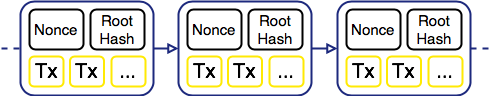
\includegraphics[width=0.7\textwidth]{images/blockchain}
    \caption{Conceptual depiction of a slice of a Bitcoin-like blockchain. Blocks contain multiple transactions and are chained together through the hash of the previous block. Source: \textit{Creation of TU Delft BLockchain Lab}}
    \label{fig:basic_blockchain}
\end{figure}

All agents are acting on the same copy of the blockchain. The one global chain therefore contains 
all transactions that happen on the network. This implies that all agents need to be informed about any new block.
In order to allow for enough time to synchronize transactions and blocks, the difficulty of the puzzle 
can be increased. This ensures a approximately fixed time between new blocks. This block time is 
10 minutes for Bitcoin. Together with the fixed block size the global transaction throughput of the
system is capped. For Bitcoin this is approximately 7 transactions per second. The Bitcoin solution
does not scale and is in its current state no possible solution for a global trust system.

\subsection{Tamper-proof}
% why?: show that the hash chain creates a tamper-proof record
By including the hash of the previous block in each new block, the blockchain creates an append-only
chain. Any slight change to any block will change the hash of that block and thus break the chain. 
Also, because every node on the network maintains the same chain, just changing one block locally 
is not enough, only new blocks on the longest chain are accepted by nodes. Thus the only way to 
actually attack the system is by mining blocks faster than the rest of the network. This is only 
possible when a majority of the network's CPU power works together which is very unlikely for very
large networks. The blockchain therefore offers a very tamper-proof solution for storing transactions
in a distributed system.

\subsection{Incentive}
% why?: 
Bitcoin-like distributed ledgers create an incentive for agents to publish new blocks by rewarding 
them with currency. New blocks are accepted if they are on top of the longest chain. This creates 
an incentive for all participating miners to stay up to date on the state of the global ledger. Only
if an agent is in possession of the latest block is there a chance to receive the block reward. 
Conflicts can arise when two blocks are found at approximately the same time. Each block will be 
considered the latest by part of the network. The conflict will be resolved once the next block is 
found in any of the two parts, creating the new longest and valid chain. Agents from the other part 
will immediately switch to the longer chain. This ultimately leads to global consensus on the 
current chain.

% Explain Sharding
% 

\section{TrustChain}
\label{sec:trustchain}
TrustChain is designed with scalability in mind. It's design focus is in stark contrast with that of
Bitcoin. Instead of employing global consensus to guarantee a single global transaction ledger, 
all agents in the TrustChain fabric are owner of a chain for themselves. This creates a scalable 
solution in which the total network throughput grows with the size of the network. However, the
scalability comes at the cost of security guarantees. This section will first discuss the general 
architecture of trust chain before discussing the scalability and some details of the implementation.

\begin{figure}
    \centering
    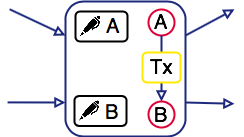
\includegraphics[width=0.35\textwidth]{images/block}
    \caption{A single block in the TrustChain fabric. Incoming arrows represent block hashes from the previous blocks of the agents' chains. Source: \textit{Creation of TU Delft BLockchain Lab}}
    \label{fig:trustchain_block}
\end{figure}

\subsection{Data structure}
\label{sec:transaction_blocks}
Blocks in TrustChain record exactly one transaction between two parties. Because both parties have 
their own chain and the transaction concerns both parties, any new block is added to both agents'
chains. Each block contains the following main elements:

\begin{itemize}
    \item \textbf{Transaction.} The actual content of the block is the data of the transaction. 
    TrustChain is designed to be application agnostic. Thus the content of a transaction can be any 
    serializable data. In the case of Tribler the transaction contains the amount of data that was
    uploaded and downloaded from the perspective of the initiator.
    \item \textbf{Previous block hashes.} The hashes of the previous blocks of both agents' chains 
    firmly attaches the new block to their history. This is similar to the basic blockchain concept.
    \item \textbf{Public Keys.} In order to uniquely identify the two agents that conduct a transaction
    their public keys are recorded.
    \item \textbf{Signatures.} Both agents provide a digital signature of the transaction with their 
    private key which any agent can check with the agents' public keys. This authenticates the 
    transaction and cryptographically proves that the real owners of the private key conducted the 
    transactions.
    \item \textbf{Sequence numbers.} All blocks on an agent's chain have a unique sequence number 
    which shows the position in the chain. 
\end{itemize}

A simplified depiction of a TrustChain block is shown in Figure~\ref{fig:trustchain_block}. When 
looking at a single agent the given data structure creates a chain of blocks which describea all the
transactions of that agent. However the second incoming and outgoing edge of each block entangles an
agent's chain with those of all partners. When looking at a complete network of the transactions the
represents a directed acyclic graph(DAG). Such a structure is shown in Figure~\ref{fig:trustchain_graph}.

\begin{figure}
    \centering
    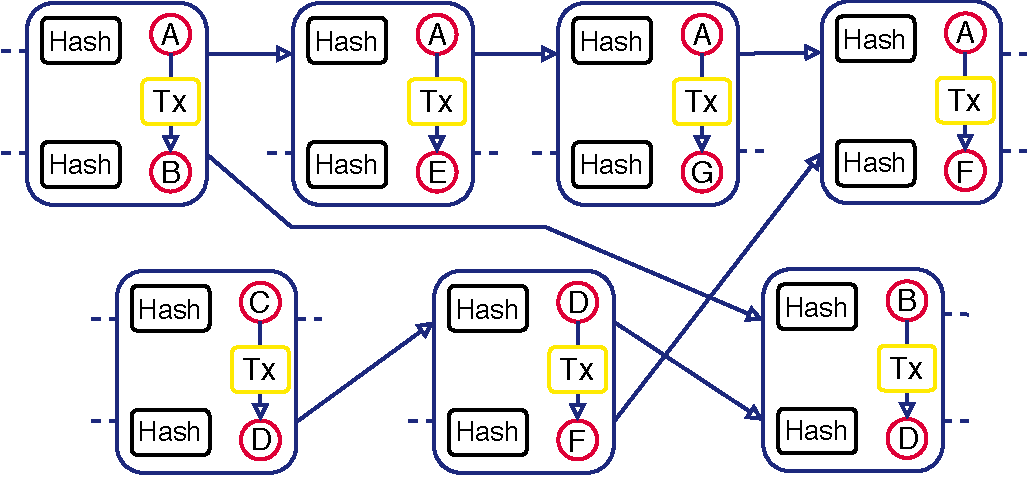
\includegraphics[width=\textwidth]{images/trustchain_graph.pdf}
    \caption{TrustChain graph structure with multiple transactions. The top row shows the chain of
    an agent A with links to multiple other blocks. Source: \textit{Creation of TU Delft BLockchain Lab}}
    \label{fig:trustchain_graph}
\end{figure}

\subsection{Scalability}
\label{sec:trustchain_scalability}
A transaction in TrustChain only requires the agreement of the two participating nodes on the content
of the block. Each node shows acceptance by digitally signing the block and returning it to the 
other party. Therefore transactions do not need to be publicly announced or sent to all nodes on
the network. Also, multiple transactions can be performed at the same time globally without breaking
the rules of the system. In contrast to the Bitcoin system, only the transactions of each agent are
strictly ordered, the global set of transactions is not.

This result is a system that scales with the size of the network. A simple example makes this very 
clear. Consider two networks, one with 10 nodes and one with 100 nodes. For simplicity we consider
time to be discrete and agents interact in rounds. Each transaction takes 1 round and all agents 
interact. Throughput calculation is then straightforward. Nodes arrange in pairs and perform a
transaction. The small network will have 5 pairs and thus 5 transactions per round, while the large
network has 50 pairs and transactions. Although this example is extremely simplified, no real-world
effect like network delays, network churn or bandwidth restrictions greatly conflict with this property.

\subsection{Security}
Similar to a single Blockchain the graph structure of TrustChain creates a tamper-proof record of
transactions. Although each user controls an own chain and can manipulate it without other agents 
noticing, any manipulation will render the signature of the transaction partner invalid. Also, all 
blocks are at least owned by two nodes. Should one agent try to hide the transaction, it will not 
completely disappear from the network because the partner still owns a copy. Therefore transactions
are still recorded in a tamper-proof data structure.

However problems arise with attacks that don't directly manipulate the data structure but make use 
of the incomplete knowledge which is intrinsic to distributed networks. A prominent example, 
double spend attack, has been defined and extensively discussed in Chapter~\ref{chap:model}. We have
shown that gossiping, that is sharing of knowledge, is a way to detect such attacks. The current
TrustChain system does not record gossiping in any way. Therefore agents do not have a strong 
incentive to perform gossiping. In the next section an extension will be discussed which adds the 
possibility of recording exchanges.

\section{Extension}
\label{sec:extension}
Proven detectability of malicious and free-riding nodes can only be attained when gossiping behavior
is recorded and incentivized. We now propose an architecture based on TrustChain which allows the 
implementation of the ordered encounter model from the previous chapter. TrustChain is extended with
\textit{exchange blocks}. They are similar to blocks that record transactions as introduced in 
Section \ref{sec:transaction_blocks} but instead of documenting a transaction it records the 
transaction of information.

\subsection{Implementation details}
Exchanges can be recorded in the same way as transaction data is recorded. Instead of the transaction
field we add an exchange field which stores the uploaded and downloaded data from the perspective of
the agent that initiates the exchange. However, exchanges can become very large, in a theoretical 
worst case the whole network's data. Therefore we do not store all exchanged blocks directly but only
the root hash of a Merkle tree of the blocks. 

\begin{figure}
    \centering
    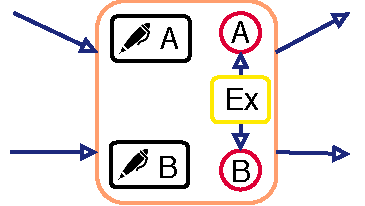
\includegraphics[width=0.35\textwidth]{images/exchange_block.pdf}
    \caption{A single exchange block for the TrustChain fabric. Source: \textit{Adpated from TU Delft BLockchain Lab}}
    \label{fig:exchange_block}
\end{figure}

Each agent keeps track of the actual set of blocks that were received in an exchange block such that 
the hash can be recalculated to check the consistency of the exchange block. Specifically, each 
node stores an index of the blocks contained in an exchange in a separate database. This index can be 
used to retrieve the actual blocks from the database of blocks. 

\subsection{Exchange process}
We shall now describe the process of an exchange between two agents in detail. We consider two honest 
agents $A$ and $B$ in a Tribler context. $A$ would like to stream a video which $B$ possesses. According
to some exchange policy, $A$ is required to exchange information with $B$ and verify it before the 
interaction can take place. Thus, $A$ initiates the exchange by sending $A$'s complete chain to $B$,
together with a block index for each exchange block.
$B$ can perform simple checks on the chain, for example whether it contains the correct exchanges 
according to the exchange policy and whether all blocks are correctly signed and chained. From the 
chain and the exchange block indexes, $B$ is able to reconstruct the complete database of $A$ which 
is the equivalent of the subjective network state from Section~\ref{sec:definitions}. 

At this point the action of $B$ depends on the actual exchange policy that is employed. According to
the Hisory-Exchange policy (see Section \ref{sec:model_double_spend}) $A$ has already provided 
enough information and $B$ will send his own chain. For the Network-State-Exchange it works a as
follows. Given $A$'s database, $B$ can calculate the difference between their databases. $B$ will 
then request from $A$ the blocks that $A$ has but $B$ does not. Once $A$ replies, $B$ has all 
information that $A$ has. $B$ is then able to recalculate all exchange hashes of $A$ to check that 
the exchange blocks are correct. If $A$'s chain completely checks out, $B$ sends his chain, exchange
indexes and blocks to $A$. Note that $B$ already knows which blocks $A$ is missing with respect to 
$B$ and can therefore directly send them. 

Now $A$ is able to perform the same checks as $B$. If $B$'s data also checks out, $A$ will create 
a new exchange block. The exchange block contains the root hash of the data that $A$ uploaded to $B$ 
and downloaded from $B$. As $B$ also knows that he downloaded from $A$ and uploaded to $A$, $B$ should
be able to calculate the same hashes. After both parties sign the block, they add them to their 
database of blocks. Also they create an entry for the exchange block in the exchange index map, which 
maps each exchange block to the index of exchanged blocks. Finally, they are able to perform the 
actual uploading and downloading of data. 

\subsection{Exchange policy flexibility}
The architecture that we have presented in this section is very flexible. Any size of information 
exchange between two parties can be recorded. It therefore allows for the implementation of any 
exchange policy. We have shown in Chapter \ref{chap:model} that the Network-State-Exchange policy
can give strong guarantees for security but also induces the highest cost on storage and bandwidth 
capacity. Depending on the application this might be necessary however TrustChain was designed to 
be as scalable as possible without global consensus. Therefore also less demanding exchange policies
can be implemented.  

\subsection{Scalability concerns}
Each exchange between agents adds an additional block to their chain. Also the blocks that the 
exchange contains need to be transmitted and stored. This increases the bandwidth and storage 
requirements, depending on the exchange policy. However, the main property of linear scalability 
still applies, at least when assuming that storage capacity is not a problem. Each exchange and 
transaction still only requires two agents to communicate, thus parallel transactions is still 
possible and the example given in Section \ref{sec:trustchain_scalability} applies in the same way.
Problems occur when we include the storage requirement. For example, the Network-State-Exchange policy
requires agents to exchange all blocks with each transaction partner. Thus each agent that periodically
interacts will approach the complete network state. Depending on the agents transaction frequency and
the network's frequency there is a considerable delay between the subjective agent's state and the
network state. Still, this will lead to storage problems if agents need to run on mobile devices or
even personal computers. 

The flexibility in exchange policy allows the system designer to ship software with a less stringent
exchange policy. This will reduce security but also reduce the requirements on storage and bandwidth.
Otherwise it should be possible to delete data. This could also be recorded on chain. As only the 
root hash of the exchanges are stored on an agents chain, a delete block should be possible by 
recording in a similar fashion without the need to remove blocks from the chain. Therefore chain 
consistency is kept intact. How this should be implemented in detail and a security analysis will 
be left for future research.

\section{Example}
In order to make the implementation more clear, an example is provided in this section. We look at two
agents, Alice and Bob. Alice wants to interact with Bob and starts the interaction. We assume that
both agents are new to the network and only have their genesis blocks on the chain. In order to
start the interaction, Alice sends her chain (only the genesis block) and an empty set of exchanges
to Bob. Obviously the genesis block is accepted and Bob shows his approval by sending his own
genesis block and an empty set of exchanges. Also Alice accepts the data and creates an exchange 
block proposal. Figure \ref{fig:exchange_example} shows the chains of Alice and Bob after the 
complete interactions. The block proposal is Alice's block 2. When Bob receives the block, he checks
that the exchange hashes in the proposed exchange block match the hashes of the two genesis blocks 
from Alice and himself. If he agrees, he documents the acquisition of the exchange block in a
single-signed exchange block (Bob's block 2) and creates the agreement block (Bob's block 3) to the exchange block proposal. He sends back the exchange block agreement to Alice, who herself creates a single-signed exchange block
(Alice's block 3) for the acquisition of the exchange agreement block. At this point Alice is ready for the actual 
transaction. How the transaction happens exactly is not of importance for this example. After the transaction was successfully conducted it also needs to be documented. Again,
the same process as with the exchange is followed. Alice creates a transaction block proposal (Alice's block 4), Bob
creates the acquisition block and the agreement block (Bob's block 4 and 5). Finally, Alice creates the acquisition block of the agreement block of the transaction.

\begin{figure}
    \centering
    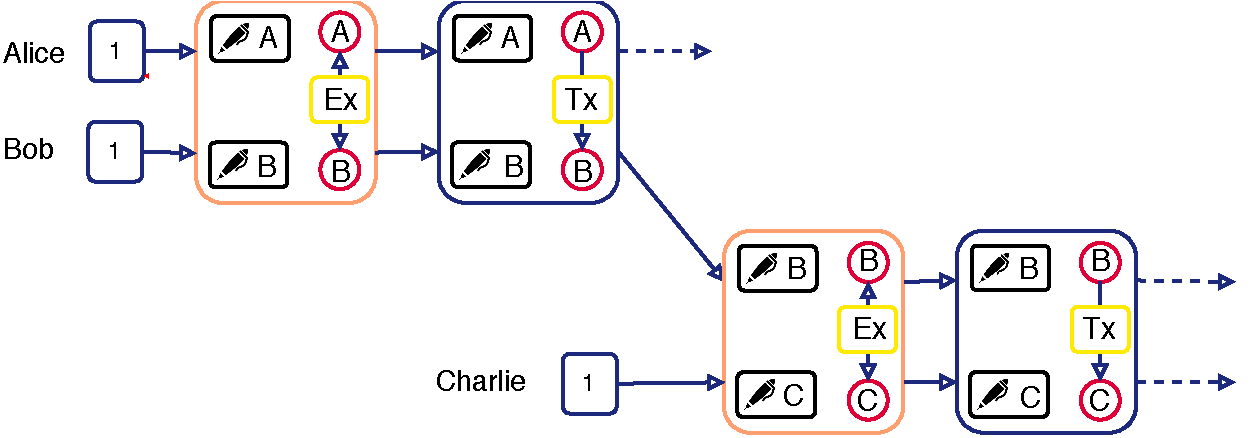
\includegraphics[width=\textwidth]{images/trustchain_example.pdf}
    \caption{Example of one interaction between three agents}
    \label{fig:exchange_example}
\end{figure}

This example sheds light on the block creation process but is too simple to properly explain the 
exchange and verification process. We extend the example with another agent, Charles, whom Bob would
like to interact with after the previous interactions. Again, Charles is assumed to be new to the 
network so the genesis block is the only block on his chain. Bob starts the interactions by sending
his chain and exchanges. Now Charlie performs some checks: 

\begin{itemize}
    \item \textit{Is the chain complete?} - the chain is a full sequence (1 through 5) and Charlie 
    is not aware of any later blocks than 5, so the chain seems valid
    \item \textit{Are the exchanges correct?} - there are three exchange blocks on the chain, one
    receiving the exchange block proposal, one for the actual exchange of the genesis block of A and
    one for the transaction block proposal. Charlie recalculates the hashes stored in the exchange 
    blocks from the blocks sent by Bob. If all the hashes are equal, the exchanges are accepted.
\end{itemize}

Once Charlie accepts all the checks, he sends his own chain and exchanges which are checked by Bob
and the interaction continues as previously described. Table \ref{tab:blocks_example} shows the
blocks that each agent has after the first and second round. After the second round, Charles has 
all the blocks from Bob that he had after the first round.

\begin{table}[h!]
    \centering
    \caption{The block databases of each agent for the example}
    \label{tab:blocks_example}
    \begin{tabular}{p{4cm}|p{3cm}|p{4cm}|p{3cm}}
        \toprule
        Database & Alice & Bob & Charles \\
        \midrule
        Before first round & A: $[1]$ & B: $[1]$ & C: $[1]$ \\ \hline 
        After first round & A: $[1, 2, 3]$ \newline B: $[1, 2, 3]$ & A: $[1, 2, 3]$ \newline B: $[1, 2, 3]$ & C: $[1]$ \\ \hline
        After second round &  A: $[1, 2, 3]$ \newline B: $[1, 2, 3]$ & A: $[1, 2, 3]$ \newline B: $[1, 2, 3, 4, 5]$ \newline C: $[1, 2, 3]$ & A: $[1, 2, 3]$ \newline B: $[1, 2, 3, 4, 5]$ \newline C: $[1, 2, 3]$ \\
        \bottomrule
    \end{tabular}
\end{table}

\section{Attacks}
\label{sec:attacks}
The model of Mui can be mapped onto the TrustChain implementation context in a straight-forward 
fashion. We showed that in TrustChain, an agent's embedded social network 
and the agent's true reputation can be inferred simply from the complete set of block that 
the agent had. Blocks are the receipt of an encounter between two agents. 

If the trust system works as expected, a good reputation should have value to agents. All agents on 
the network attempt to obtain a good reputation and be seen as a trusted partner. As such their 
behavior should be meticulously agree with the rules. Yet, if the value is large enough and behaving
well comes at a large enough cost, agents will aim to bend the rules or even break them in a smart 
way in order to get the good reputation for free. As a designer of the trust system it is essential
to predict the possible ways of manipulation and prevent them. In this section we will define several
known types of attacks on trust systems and if applicable define how TrustChain can prevent them.

\subsection{Forking}
Forking is one of the most well-known attacks of blockchain based systems. In the cryptocurrency 
context it is also known as double spending. As defined in Definition \ref{def:fork} an attacking agent 
sends two conflicting transactions to two different partners. As long as the two partners are each not 
aware of the other version of the transaction, both transactions are accepted. This practically 
allows the attacker to reuse some reputation that normally would already have been lost or overwrite
a transaction that would otherwise lower the attacker's reputation.

The fact that agents in the TrustChain fabric are solely responsible for their own chain forking is
easy and cannot be prevented. However in certain circumstances the attack can be detected, putting a
negative mark on the attacker. Namely, if one of the agents who were subject to the attack learn 
about the other version of the block, they can see that the attacker signed two conflicting blocks.
This creates a proof-of-fraud and the agent can ignore the attacker in the future. 

\subsection{Transaction hiding}
Once agents have a longer history they will have records of positive and negative encounters. A 
malicious agent then might try to hide any records of negative encounters, thus boosting the trust 
other have in the attacker. The architecture of TrustChain is made to make such an attack detectable.
The blockchain of the agent creates a tamper-proof, irreversible order for all transactions. Another
agent can therefore require the complete sequence of blocks of a partner before interacting. Any 
missing block will be seen as a malicious request. 

The attack can also be mitigated if the partners of the attacker, who also own the blocks that proof
the negative encounters of the attacker, disseminate that information to their peers. As such agents
may already know about the true reputation of the attacker and decide to ignore that agent in the 
first place.

\subsection{Whitewashing}
Agents that have lost reputation in a significant amount of transaction may decide to create a new 
identity for themselves. Thus they can rid themselves from the bad reputation and start fresh. This 
type of attack is called whitewashing. In the currently deployed version of TrustChain in Tribler 
this attack cannot be prevented as the software is free and new agents do not need registering with
any central institutions.

Still the impact of such attacks can be limited by having some mistrust of new agents joining the 
network. In that case a new agents need to ``pay their dues'' before being accepted by the network 
as equals.

\subsection{Sybil attack}
One of the most serious attacks on trust systems is the Sybil attack. In a Sybil attack the attacker
creates a set of new accounts, called the Sybils. Together with the attacking agent the set of 
agents is called a Sybil region. Those Sybils create transaction records 
between each other without actually performing the transactions with the goal of boosting the 
reputation of one of the agents in the Sybil region. The attack is successful as honest agents 
cannot distinguish between fake and real transaction records. That also makes the attack hard to 
prevent.

Multiple ways have been explored to prevent this attack. One way is to analyze the network topology
and use it to detect Sybil regions. Another way is to increase the cost of registering new identities
in the system. 

\subsection{Other attacks}
Other obvious attacks are for example a direct tampering with a block. Such attacks can be 
detected in a straightforward way by simply recalculating the hash and checking with the following 
block and the signature of the agents.


\section{System level trust}
* Verification and exchanges make an agent trustworthy on a system level, as in, we trust them to 
stick to the rules of recording, exchanging and verifying
* Use this to not verify each and every agent, but assume agent which were verified by trustworthy
agents to be trustworthy enough for interaction
* At every point we still have the chance to do the complete verification of a history. But maybe 
its not required every turn